%%
%% This is file `sample-sigconf.tex',
%% generated with the docstrip utility.
%%
%% The original source files were:
%%
%% samples.dtx  (with options: `all,proceedings,bibtex,sigconf')
%%
%% IMPORTANT NOTICE:
%%
%% For the copyright see the source file.
%%
%% Any modified versions of this file must be renamed
%% with new filenames distinct from sample-sigconf.tex.
%%
%% For distribution of the original source see the terms
%% for copying and modification in the file samples.dtx.
%%
%% This generated file may be distributed as long as the
%% original source files, as listed above, are part of the
%% same distribution. (The sources need not necessarily be
%% in the same archive or directory.)
%%
%%
%% Commands for TeXCount
%TC:macro \cite [option:text,text]
%TC:macro \citep [option:text,text]
%TC:macro \citet [option:text,text]
%TC:envir table 0 1
%TC:envir table* 0 1
%TC:envir tabular [ignore] word
%TC:envir displaymath 0 word
%TC:envir math 0 word
%TC:envir comment 0 0
%%
%%
\documentclass[sigconf,review,anonymous,screen]{acmart}

%%
%% \BibTeX command to typeset BibTeX logo in the docs
\AtBeginDocument{%
  \providecommand\BibTeX{{%
    Bib\TeX}}}

%% Rights management information.  This information is sent to you
%% when you complete the rights form.  These commands have SAMPLE
%% values in them; it is your responsibility as an author to replace
%% the commands and values with those provided to you when you
%% complete the rights form.
\setcopyright{acmlicensed}

\copyrightyear{2026}
\acmYear{2026}
\acmDOI{10.1145/XXXXXXX.XXXXXXX}
%% These commands are for a PROCEEDINGS abstract or paper.
\acmConference[CCS '26]{Proceedings of the 2026 ACM Conference on Computer and Communications Security}{November 15--19, 2026}{The Hague, The Netherlands}

\acmISBN{978-1-4503-XXXX-X/2018/06}

%%
%% Submission ID.
%% Use this when submitting an article to a sponsored event. You'll
%% receive a unique submission ID from the organizers
%% of the event, and this ID should be used as the parameter to this command.
%%\acmSubmissionID{123-A56-BU3}

\usepackage{xspace}
\usepackage{url}
\usepackage{hyperref}
\usepackage{enumitem} % For better list formatting
\usepackage{mdframed}
\usepackage{booktabs}
\usepackage{multirow}
\usepackage{algorithm}
\usepackage{graphicx}
\usepackage{esvect}

\usepackage{xcolor}
\usepackage[cache=false]{minted}
\usemintedstyle{default}
\usepackage{etoolbox}

\usepackage[noend]{algpseudocode}
\usepackage{mathtools} % Added for better math layouts

\setlist[itemize]{leftmargin=2em}
\setlist[enumerate]{leftmargin=2em}

\usepackage{tikz}
\usetikzlibrary{positioning}
\usepackage{pgfplots}
\pgfplotsset{compat=1.18}

% Math operators
\DeclareMathOperator*{\argmax}{arg\,max}

\usepackage{placeins}
\usepackage{colortbl}
\definecolor{RoyalBlue}{RGB}{65, 105, 225}
\definecolor{Orange}{RGB}{255, 165, 0}
\definecolor{Teal}{rgb}{0.0, 0.5, 0.5}
\definecolor{bluegray}{rgb}{0.4, 0.6, 0.8}
\definecolor{antiquebrass}{rgb}{0.8, 0.58, 0.46}
\definecolor{amethyst}{rgb}{0.6, 0.4, 0.8}
\definecolor{darkpastelgreen}{rgb}{0.01, 0.75, 0.24}

\renewcommand{\tablename}{Table}

\def\sectionautorefname{Section}
\def\subsectionautorefname{Section}
\def\algorithmautorefname{Algorithm}
\def\figureautorefname{Figure}
\def\tableautorefname{Table}
\def\equationautorefname{Equation}

\newcommand{\tool}{$\textsc{Beak}$\xspace}
\newcommand{\zkap}{$\textsc{ZKap}$\xspace}
\newcommand{\arguzz}{$\textsc{Arguzz}$\xspace}
\newcommand{\circomspect}{$\textsc{Circomspect}$\xspace}
\newcommand{\yanju}[1]{{{\color{blue}{{(Yanju: #1)\xspace}}}}}
\newcommand{\yu}[1]{{{\color{red}{{(Yu: #1)\xspace}}}}}
\newcommand{\tbd}[1]{{{\color{red}{{{\bf #1}\xspace}}}}}

\definecolor{hlcolor}{HTML}{156082}
\newcommand{\hl}[1]{{{\color{hlcolor}{#1\xspace}}}}

\newcommand{\imidrule}{\specialrule{0pt}{0.2em}{0.2em}}

\newcommand{\reducedstrut}{\vrule width 0pt height .1\ht\strutbox depth .1\dp\strutbox\relax}
\newcommand{\irule}[1]{%
  \begingroup
  \setlength{\fboxsep}{0pt}%
  \colorbox{RoyalBlue!15}{\reducedstrut(#1)\/}%
  \endgroup
}

\newcommand{\icode}[1]{%
  \begingroup
  \setlength{\fboxsep}{0pt}%
  \colorbox{gray!20}{\reducedstrut\texttt{\small{#1\xspace}}\/}%
  \endgroup
}

%%
%% end of the preamble, start of the body of the document source.
\begin{document}
\sloppy

%%
%% The "title" command has an optional parameter,
%% allowing the author to define a "short title" to be used in page headers.
\title{Revealing Semantic Gaps in Zero-Knowledge Virtual Machines via Invariant-Targeted Semantic Fuzzing}

%%
%% The "author" command and its associated commands are used to define
%% the authors and their affiliations.

\author{Hongbo Wen}
\email{hongbowen@ucsb.edu}
\affiliation{%
  \institution{University of California, Santa Barbara}
  \city{Santa Barbara}
  \state{CA}
  \country{USA}
}

% \author{Author Two}
% \email{author2@example.com}
% \affiliation{%
%   \institution{Example University}
%   \city{City}
%   \state{State}
%   \country{Country}
% }

%%
%% By default, the full list of authors will be used in the page
%% headers. Often, this list is too long, and will overlap
%% other information printed in the page headers. This command allows
%% the author to define a more concise list
%% of authors' names for this purpose.
% \renewcommand{\shortauthors}{Wen et al.}

%%
%% The abstract is a short summary of the work to be presented in the
%% article.
\begin{abstract}

Zero-knowledge virtual machines (zkVMs) prove correct execution of RISC-V programs, but their security depends on faithful alignment between the RISC-V specification and the arithmetization that certifies an execution trace. When this alignment breaks, a prover can forge proofs for incorrect executions, undermining the trust model of systems securing billions of dollars. Detecting such \emph{semantic gaps} is challenging: each zkVM encodes its trace differently, and bugs cluster at rare boundary conditions that are effectively unreachable by random testing.

Our key insight is that soundness bugs in zkVMs fall into two structurally distinct classes---executor \emph{divergences} and constraint \emph{underconstraints}---and that, despite heterogeneous internal representations, the boundary conditions triggering both classes are shared across backends. We present \tool, a semantics-guided differential fuzzing framework that exploits this structure. \tool defines a \emph{cross-zkVM semantic model} that lifts six production backends into a common space of 17 observation types and 32 semantic categories, and builds a \emph{boundary-driven fuzzing framework} where category signature novelty replaces edge coverage, a multi-armed bandit governs eight ISA-aware mutation strategies, and semantic witness injection probes underconstrained circuits at identified boundary points. We establish a two-phase coverage characterization showing that the detection phases are complementary: neither subsumes the other, and removing witness injection reduces recall from 81.8\% to at most 11.4\%.

Evaluated across OpenVM, SP1, RISC Zero, Jolt, Nexus, and Pico on 44 known vulnerabilities, \tool achieves 81.8\% recall (36/44). On the four backends where the prior state-of-the-art (Arguzz) has full support, \tool detects 1.6$\times$ more bugs (18 vs.\ 11); across all six backends, the improvement is 3.3$\times$ (36 vs.\ 11). \tool additionally discovers 6 previously unknown zero-day vulnerabilities including critical soundness violations in production systems. All findings have been responsibly disclosed and patched.

\end{abstract}


%%
%% The code below is generated by the tool at http://dl.acm.org/ccs.cfm.
%% Please copy and paste the code instead of the example below.
%%
\begin{CCSXML}
<ccs2012>
   <concept>
       <concept_id>10002978.10003022.10003023</concept_id>
       <concept_desc>Security and privacy~Software security engineering</concept_desc>
       <concept_significance>500</concept_significance>
       </concept>
   <concept>
       <concept_id>10011007.10011074.10011099.10011102</concept_id>
       <concept_desc>Software and its engineering~Software testing and debugging</concept_desc>
       <concept_significance>500</concept_significance>
       </concept>
   <concept>
       <concept_id>10002978.10003014.10003017</concept_id>
       <concept_desc>Security and privacy~Formal methods and theory of security</concept_desc>
       <concept_significance>300</concept_significance>
       </concept>
 </ccs2012>
\end{CCSXML}

\ccsdesc[500]{Security and privacy~Software security engineering}
\ccsdesc[500]{Software and its engineering~Software testing and debugging}
\ccsdesc[300]{Security and privacy~Formal methods and theory of security}

%%
%% Keywords. The author(s) should pick words that accurately describe
%% the work being presented. Separate the keywords with commas.
\keywords{Zero-Knowledge Proofs, Fuzzing, Virtual Machines, Semantic Gaps}

%%
%% This command processes the author and affiliation and title
%% information and builds the first part of the formatted document.
\maketitle

\section{Introduction}\label{sec:intro}

Zero-knowledge virtual machines (zkVMs) enable a prover to execute arbitrary RISC-V programs and produce succinct cryptographic proofs of correct execution~\cite{risc0, sp1, jolt}. Production deployments already underpin blockchain scaling solutions, privacy-preserving applications, and off-chain computation platforms securing billions of dollars in digital assets~\cite{openvm, nexus, pico}. The security of these deployments hinges on a critical invariant: the zkVM's arithmetization---the polynomial constraints encoding the execution trace---must faithfully capture the RISC-V instruction semantics. When this alignment fails, a malicious prover can forge proofs for incorrect executions, undermining the entire trust model.

Detecting such \emph{semantic gaps} is extremely challenging. The constraint systems are large (hundreds of thousands of constraints), component interactions are subtle (e.g., the ALU must agree with the memory subsystem on the value written to a register), and bugs manifest only under specific \emph{boundary conditions}: rare combinations of operand values, instruction orderings, and execution states that exercise edge cases in the arithmetization. These bugs rarely surface during normal testing or standard security audits.

Existing approaches fall short. Static analysis tools such as \zkap~\cite{zkap} detect generic patterns (e.g., unconstrained signals) but lack zkVM-specific semantic structure, producing high false positive rates while missing actual bugs. Dynamic approaches such as \arguzz~\cite{arguzz} combine metamorphic testing with fault injection, but rely on generic mutation strategies unlikely to reach the boundary conditions where constraint bugs hide; in our experiments, \arguzz times out on the majority of benchmarks. Both lack a \emph{semantic model} of what constitutes a boundary condition and how to explore these conditions across heterogeneous backends.

Our key insight is that soundness-critical gaps in zkVMs arise at \emph{semantic boundary conditions} that become observable when heterogeneous backend traces are \emph{lifted into a common semantic space}. Although each zkVM represents its execution trace differently, the constraint-correctness concerns they share---immediate value decomposition, memory address alignment, control flow target binding, arithmetic overflow handling---can be captured by a small, well-defined set of semantic categories. Moreover, the bugs that these categories identify fall into two fundamentally distinct classes: \emph{divergences} (the executor computes incorrectly) and \emph{underconstraints} (the executor is correct but the constraint system is too permissive). Detecting both classes requires complementary mechanisms, a property we formalize as \emph{two-phase coverage} (\autoref{sec:formal-properties}). By naming semantic categories and using them as a structured feedback signal, a fuzzer can systematically explore the semantic dimensions where bugs cluster, rather than blindly mutating inputs.

Based on this insight, we introduce \tool, a semantics-guided differential fuzzing framework for discovering constraint bugs in RISC-V zkVMs. \tool makes two core contributions. First, it defines a \emph{cross-zkVM semantic model} that unifies six heterogeneous zkVM backends (OpenVM, SP1, RISC Zero, Jolt, Nexus, and Pico) into a common space of 17 observation types and 32 semantic categories, enabling cross-backend constraint-correctness reasoning without per-backend analysis (\autoref{sec:trace-ir}). Second, it builds a closed-loop \emph{boundary-driven fuzzing framework} on this shared abstraction: category signature novelty replaces edge coverage as the feedback signal, a UCB1 multi-armed bandit governs eight ISA-aware mutation strategies, and semantic witness injection probes underconstrained circuits at identified boundary points (\autoref{sec:fuzzing-framework}).

We evaluate \tool on all six backends against a ground-truth benchmark of 44 known vulnerabilities sourced from zero-day discovery, prior dynamic testing, security audits, and public issue trackers. \tool detects 36 of 44 bugs (81.8\% recall). On the four backends where Arguzz~\cite{arguzz} has full support, \tool detects 18 bugs to Arguzz's 11 (1.6$\times$); across all six backends, the improvement is 3.3$\times$ (36 vs.\ 11, 25.0\%). \tool additionally discovers 6 previously unknown zero-day vulnerabilities, including 3 critical soundness bugs in RISC Zero, OpenVM, and Pico that allow forging proofs for incorrect RISC-V execution. All zero-day vulnerabilities have been responsibly disclosed to the respective development teams.

In summary, we contribute:
\begin{itemize}
    \item A \textbf{cross-zkVM semantic model} of 17 observation types and 32 semantic categories that unifies six backends, with a formal two-phase coverage characterization (\autoref{sec:trace-ir}, \autoref{sec:formal-properties}).
    \item A \textbf{boundary-driven fuzzing framework} with category-signature feedback, bandit-guided ISA-aware mutation, and semantic witness injection (\autoref{sec:fuzzing-framework}).
    \item A \textbf{comprehensive evaluation} achieving 81.8\% recall on 44 known bugs ($3.3\times$ over the state-of-the-art) and 6 zero-day discoveries (\autoref{sec:eval}). We will open-source \tool upon acceptance.
\end{itemize}

\section{Background}\label{sec:background}

\subsection{Zero-Knowledge Virtual Machines}\label{sec:bg-zkvm}

A zero-knowledge virtual machine (zkVM) enables a \emph{prover} to execute a program and produce a succinct cryptographic proof of correct execution, which a \emph{verifier} checks without re-executing. RISC-V is the dominant zkVM ISA; production systems include OpenVM~\cite{openvm}, SP1~\cite{sp1}, RISC Zero~\cite{risc0}, Jolt~\cite{jolt}, Nexus~\cite{nexus}, and Pico~\cite{pico}.

\paragraph{Execution pipeline}
A RISC-V zkVM processes a program through four stages: (1)~\emph{execution} produces a trace recording registers, memory, and internal signals at each step; (2)~\emph{trace generation} organizes rows as an Algebraic Intermediate Representation (AIR) or Randomized AIR with Preprocessing (RAP); (3)~\emph{arithmetization} encodes the trace as polynomial constraints over a finite field---e.g., an \icode{add} instruction requires the destination column to equal the sum of source columns modulo the field prime; and (4)~\emph{proof generation} via a polynomial commitment scheme (FRI or KZG) produces a proof the verifier checks in polylogarithmic time.

\paragraph{Key components}
A typical trace comprises an \emph{instruction decoder} (correct field extraction from 32-bit words), an \emph{ALU} (arithmetic/logic with limb decomposition), a \emph{memory subsystem} (load/store consistency), \emph{lookup tables} (range checks, XOR), and \emph{cross-component interactions} (e.g., ALU output matches register write-back).

\subsection{Challenges in zkVM Vulnerability Detection}\label{sec:bg-challenges}

\paragraph{Semantic heterogeneity}
Each zkVM encodes RISC-V semantics differently: OpenVM uses modular chips with bus arguments, SP1 uses a monolithic STARK machine, and Jolt replaces arithmetization with lookup-based verification. A detection approach for one backend does not transfer.

\paragraph{Boundary conditions}
Constraint bugs cluster at \emph{semantic boundary conditions}---limb-crossing immediates, address-space boundaries, division by zero, signed overflow---that are rare in typical executions and hard to reach by random testing.

\paragraph{Oracle gap}
A zkVM's output cannot serve as ground truth (a soundness bug means incorrect executions verify), so an external reference executor must establish correct RISC-V semantics.

\subsection{Threat Model}\label{sec:bg-threat}

We adopt a \emph{malicious prover} model: the prover knows the zkVM source, witness generation, and constraint system, and aims to produce a proof accepted by an honest verifier for an execution trace deviating from correct RISC-V semantics.

\paragraph{Soundness}
Let $O$ denote a reference RISC-V oracle and $B$ a zkVM backend with arithmetization $A$ over $\mathbb{F}_p$. Backend $B$ is \emph{sound} if, for all efficient provers and inputs $x$, any accepted proof encodes a valid execution of $x$ under $O$. A \emph{soundness bug} is an input $x$ with a witness $w$ such that $A(w)$ accepts but $w$ encodes a register state $r \neq O(x)$. Our definition targets \emph{knowledge soundness}: Type~II bugs (\autoref{sec:formal-properties}) mean the constraint system is too permissive, not that the IOP or PCS is broken. \tool targets bugs in the arithmetization $A$, not the proof backend; the six backends use three distinct proof systems (FRI-based STARKs, Plonky3-based STARKs, Lasso-based lookups), but constraint-level bugs are independent of the proof backend.

\paragraph{ISA scope}
\tool models RV32IM as specified in the RISC-V ISA manual~\cite{riscvspec}. Misaligned accesses trap; division follows the spec exactly (division by zero yields $-1$/dividend; signed overflow $-2^{31} \div -1$ yields $-2^{31}$/$0$). These corner cases are where several benchmark bugs manifest (\autoref{sec:eval-rq1}). We target soundness vulnerabilities---missing constraints, incorrect constraints, and cross-component inconsistencies---not completeness bugs or performance issues.

\section{Overview}\label{sec:overview}

This section provides a high-level overview of \tool. We describe the framework architecture (\autoref{sec:framework-overview}), walk through a motivating example (\autoref{sec:motivating-example}), and state the problem formally (\autoref{sec:problem-statement}).

\begin{figure}
    \centering
    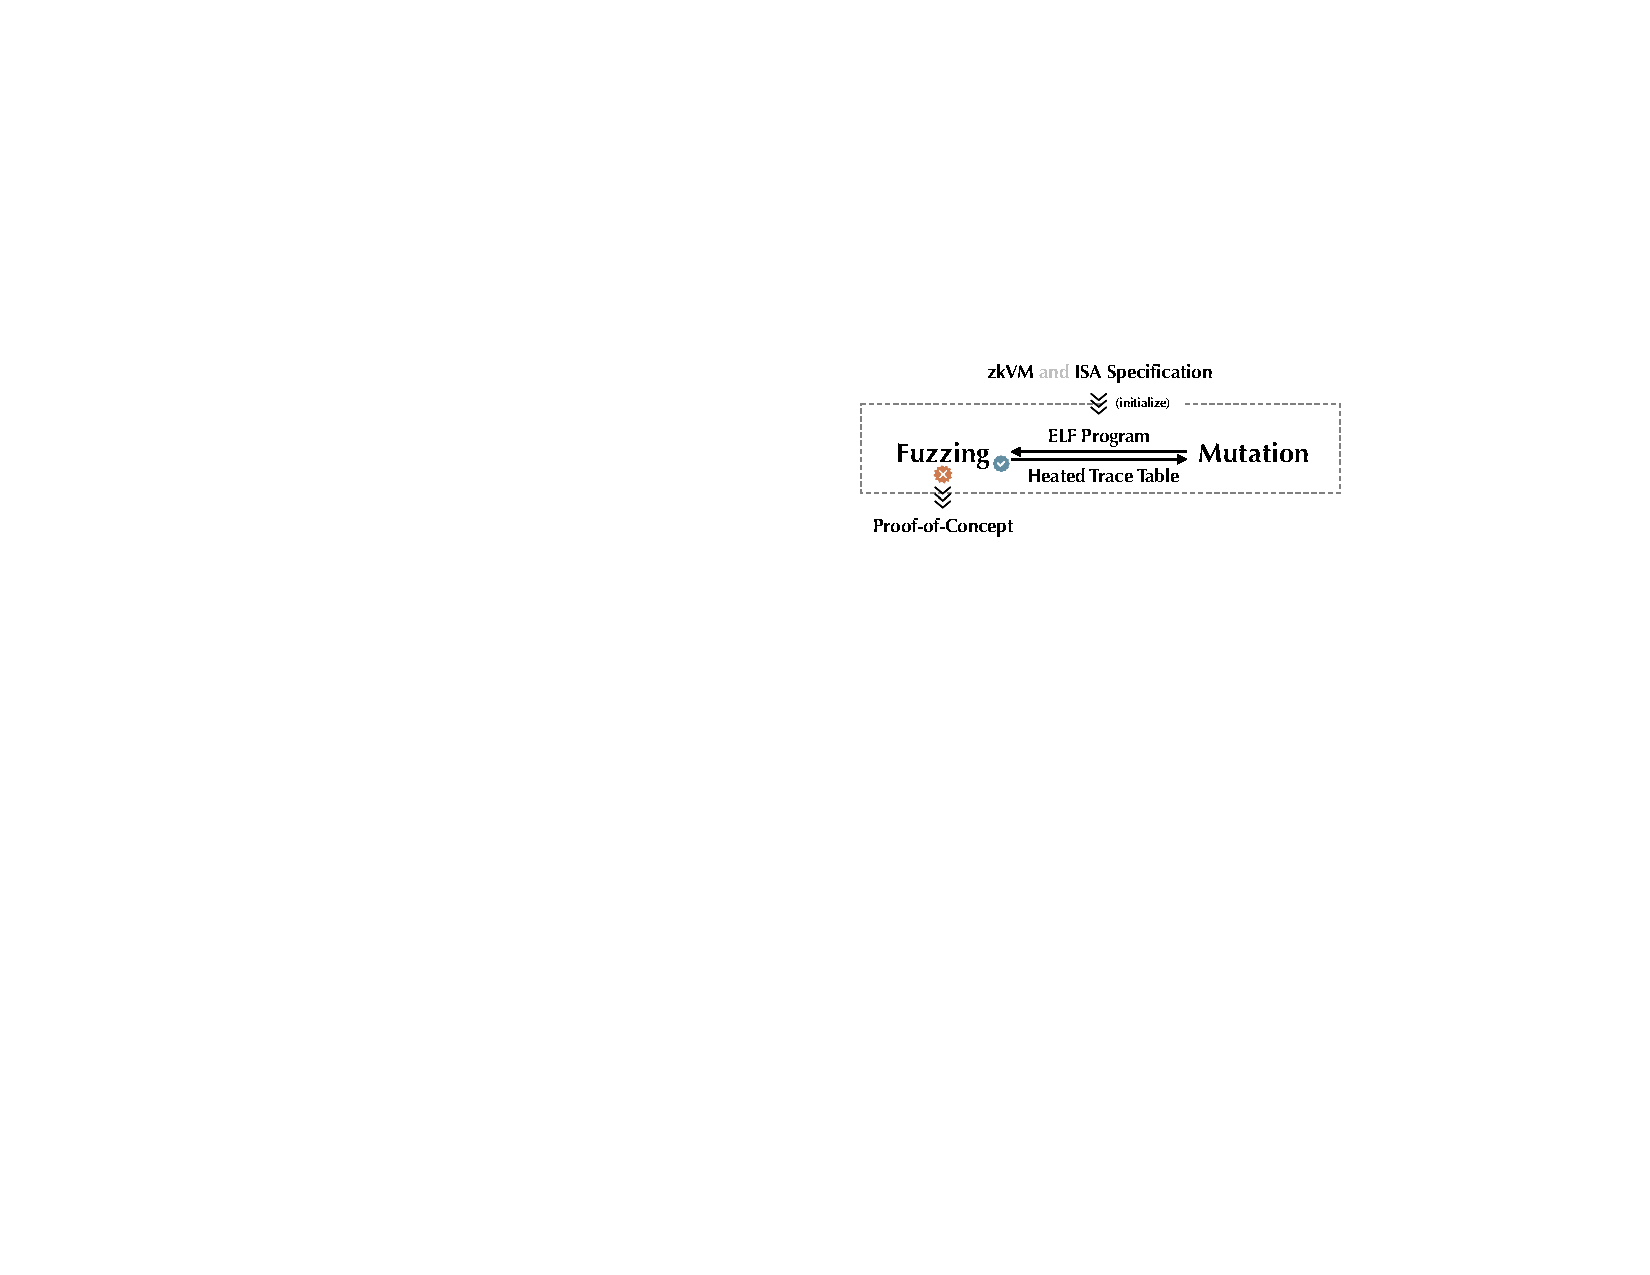
\includegraphics[width=\linewidth]{figs/overview.pdf}
    \caption{Architecture of \tool. Phase~1 performs signature-guided mutational fuzzing: RISC-V instruction sequences are mutated by an ISA-aware bandit, executed on both a reference oracle and the target zkVM backend, and projected through the semantic model to produce category signatures that guide further mutation. Phase~2 applies witness injection at constraint steps identified by the semantic model, detecting underconstrained circuits. Dashed arrows indicate feedback signals.}
    \label{fig:overview}
\end{figure}

\subsection{Framework Overview}\label{sec:framework-overview}

\autoref{fig:overview} illustrates the end-to-end architecture of \tool, which comprises two components. A \emph{cross-zkVM semantic model} (\autoref{sec:trace-ir}) lifts each backend's heterogeneous trace representation into a common vocabulary of constraint-correctness concerns, and a \emph{boundary-driven fuzzing framework} (\autoref{sec:fuzzing-framework}) uses that vocabulary to steer input generation toward underexplored boundary conditions.

The data flow proceeds as follows. A RISC-V instruction sequence is executed on both a reference oracle and the target zkVM backend. The backend's trace is projected through the semantic model to produce a \emph{category signature}: the set of constraint-correctness concerns activated by that execution. In \emph{Phase~1}, signature novelty replaces edge coverage as the fuzzing feedback signal, driving a UCB1 bandit that selects among eight ISA-aware mutation strategies. In \emph{Phase~2}, \tool probes each activated concern via targeted \emph{witness injection}, modifying the backend's internal witness to test whether the constraint system is underconstrained. The following example illustrates both phases on a real bug.

\subsection{Motivating Example}\label{sec:motivating-example}

We illustrate \tool's approach with a real constraint bug discovered in OpenVM's ALU chip: an \emph{immediate limb consistency} violation that allows a prover to decompose an immediate value into arbitrary limbs without constraint enforcement.

\paragraph{Background: immediate limb decomposition}
In OpenVM, the ALU chip processes each RISC-V instruction's immediate value by decomposing it into multiple limbs, i.e., small field elements whose product with appropriate powers of a base reconstructs the original value. For a 12-bit signed immediate (as in I-type instructions like \icode{addi}), the decomposition splits the value into byte-sized limbs. The circuit enforces a \emph{recomposition constraint}:
\begin{equation}\label{eq:recomp}
\mathit{limb}_0 + \mathit{limb}_1 \cdot 256 = \mathit{immediate}
\end{equation}
For instance, the immediate $-1$ (encoded as \icode{0xFFF} in the 12-bit two's complement) decomposes as $(\mathit{limb}_0, \mathit{limb}_1) = (\texttt{0xFF}, \texttt{0x0F})$, satisfying \autoref{eq:recomp}. To ensure a \emph{unique} decomposition, each limb must additionally be constrained to $[0, 255]$ via a range-check constraint:
\begin{equation}\label{eq:range}
0 \leq \mathit{limb}_i < 256 \quad \text{for each limb } i
\end{equation}

\paragraph{The bug}
Consider the instruction \icode{addi x1, x0, -1}, which sets register \icode{x1} to $-1$ (i.e., \icode{0xFFFF\_FFFF} in unsigned 32-bit representation). OpenVM's ALU chip enforced the recomposition constraint (\autoref{eq:recomp}) but \emph{omitted} the range-check constraint (\autoref{eq:range}) on the upper limb. This means the alternative decomposition $(\texttt{0xFF}, \texttt{0x1F})$ also satisfies the recomposition: $\texttt{0xFF} + \texttt{0x1F} \cdot 256 = \texttt{0x1FFF} \neq \texttt{0xFFF}$. Because the circuit uses the recomposed immediate to compute the instruction result, a malicious prover could claim that \icode{addi x1, x0, -1} stored a value derived from \icode{0x1FFF} rather than \icode{0xFFF}, forging a proof for an execution that never happened. The fix adds \icode{range\_check(limb\_i, 8)} for all limbs in the decomposition.

\paragraph{How \tool discovers this bug}
\tool's constant mutation arm (Arm~2) replaces an immediate with $-1$, a boundary value it prioritizes. The instrumented backend emits an \icode{ImmediateLimbObservation}, classified under \icode{alu.imm\_limb}. If this produces a novel category signature, the input enters the corpus. In Phase~2, \tool arms an injection replacing the limb values with an alternative decomposition and observes that the circuit accepts---confirming an \emph{underconstrained candidate}. The reference oracle simultaneously reports the correct value (\icode{0xFFFF\_FFFF}); the mismatch under the injected witness is recorded as a bug.

\paragraph{Why existing approaches miss this bug}
Generic fuzzing (\arguzz) is unlikely to generate immediate $-1$ \emph{and} exercise the specific ALU path; static analysis (\zkap) lacks trace-table structure to reason about limb consistency. \tool succeeds because (1)~ISA-aware mutation targets boundary immediates, (2)~the semantic model names this condition via \icode{alu.imm\_limb}, and (3)~witness injection validates constraint soundness directly.

\subsection{Problem Statement}\label{sec:problem-statement}

We now state the problem that \tool addresses.

\paragraph{Setting}
Let $O$ denote a reference RISC-V oracle that faithfully implements the RV32IM instruction set, and let $B$ denote a zkVM backend with arithmetization $A$. Given a RISC-V instruction sequence $x = (\iota_1, \ldots, \iota_n)$ where each $\iota_i$ is a 32-bit instruction word, $O(x)$ and $B(x)$ each produce a final register state $r \in \mathbb{Z}_{2^{32}}^{32}$ (a vector of 32 unsigned 32-bit integers).

\paragraph{Goal}
Find inputs $x$ such that either:
\begin{enumerate}
    \item \textbf{Semantic divergence:} $O(x) \neq B(x)$, indicating that the backend's execution trace corresponds to a different computation than the RISC-V specification prescribes; or
    \item \textbf{Underconstrained circuit:} there exists a witness injection $I_{b,s}$ (for some category $b$ and step $s$) such that $B$ accepts the altered witness without error, indicating that the arithmetization $A$ is insufficiently constrained at the boundary condition identified by category $b$.
\end{enumerate}

\paragraph{Challenges}
The search space is exponentially large, divergences occur at rare boundary conditions unreachable by random testing, and heterogeneous trace representations preclude a single testing methodology (\autoref{sec:bg-challenges}). \tool addresses these via the semantic model (unifying traces) and boundary-driven fuzzing (steering exploration).

\section{Cross-zkVM Trace Semantics}\label{sec:trace-ir}

Although each zkVM encodes its execution trace in a radically different format (chip-level AIR rows in OpenVM, STARK columns in SP1, circuit tables in RISC Zero, lookup sequences in Jolt), all these systems must enforce the \emph{same} RISC-V semantic invariants. Register x0 must remain zero. Immediate values must decompose into correctly range-checked limbs. Memory timestamps must increase monotonically. When a backend's constraint system fails to enforce one of these invariants, a soundness bug exists.

This observation is the foundation of \tool's semantic model. Rather than analyzing each backend's constraint system directly---which would require six separate analyses---we define a common vocabulary of \emph{constraint-correctness concerns}: the semantic invariants all backends must enforce. The model operates at two granularities: \emph{observations} extract structured facts from individual trace steps, and \emph{semantic categories} classify these facts into named classes of constraint behavior where bugs cluster.

\subsection{Observations and Semantic Categories}\label{sec:semantic-model}

\paragraph{Observations}
An observation is a structured fact that \tool extracts from a backend's execution trace at a specific step. Each observation records the step index, the backend component that produced it, and type-specific fields (e.g., register indices, immediate values, memory addresses). Critically, observations are \emph{backend-agnostic}: the same observation type captures the same semantic fact regardless of whether it was extracted from OpenVM's chip rows or SP1's STARK columns.

\paragraph{Running example}
Consider \icode{addi x1, x0, -1} executed on OpenVM. The ALU chip decomposes the 12-bit immediate ($-1$, encoded as \icode{0xFFF}) into byte-sized limbs for constraint evaluation over a finite field. \tool extracts an \icode{ImmediateLimb} observation recording the chip name, step index, and immediate value. The same observation type applies when SP1 or any other backend processes the same instruction; the observation abstracts away how each backend internally represents the decomposition.

More formally, an observation is a triple $o = (\tau, s, \phi)$ where $\tau \in \mathcal{T}$ is one of 17 observation types (e.g., \icode{ImmediateLimb}, \icode{ZeroRegisterWrite}), $s \in \mathbb{N}$ is the trace step index, and $\phi$ is a type-specific payload (register index, immediate value, memory address, etc.). For instance, the running example produces $o = (\texttt{ImmediateLimb},\; 42,\; \{{\tt chip}{=}\texttt{BaseAluChip},\; {\tt imm}{=}\texttt{0xFFF}\})$.

\paragraph{Semantic categories}
Observations alone do not indicate \emph{where} bugs are likely to manifest. To provide this structure, \tool classifies observations into \emph{semantic categories}, each naming a specific constraint-correctness concern. A category $c \in \mathcal{C}$ is associated with a predicate $\kappa_c : \mathcal{O} \to \{0, 1\}$ that determines whether an observation activates it. For example, the \icode{alu.imm\_limb} category activates whenever $\tau = \texttt{ImmediateLimb}$ and the immediate value crosses a limb boundary. The \emph{category signature} for input $x$ is then the set of all activated categories:
\begin{equation}\label{eq:signature}
\sigma(x) = \bigl\{c \in \mathcal{C} \;\big|\; \exists\, o \in \mathit{Obs}(x) : \kappa_c(o) = 1\bigr\}
\end{equation}
where $\mathit{Obs}(x)$ denotes the set of observations emitted by the backend during execution of input $x$ (not to be confused with the reference oracle $O$). As we describe in \autoref{sec:fuzzing-framework}, signature novelty ($\sigma(x) \notin \mathit{Seen}$) serves as the feedback signal for the fuzzing loop.

We derive our categories from a systematic analysis of three sources: (1) 25 professional security audit findings across 6 production zkVMs, (2) 11 known bugs from prior dynamic testing~\cite{arguzz}, and (3) the RISC-V RV32IM specification's boundary cases. We mapped each known bug to the constraint component it violates and abstracted recurring patterns into named categories. \autoref{tbl:categories} summarizes the result: 10 category groups spanning the major functional components of a RISC-V zkVM. As validation, all 6 zero-day vulnerabilities \tool discovered map to existing categories; no new categories were needed (\autoref{sec:eval-rq3}).

\paragraph{Category completeness and extensibility}
The 32 categories are empirically derived, not formally complete. Empirical sufficiency is validated by 97\% category activation on known bugs (\autoref{sec:eval-rq3}) and all 6 zero-days mapping to existing categories. The set is incrementally extensible: adding a category requires only a new predicate $\kappa_c$ on existing observation types---no changes to the fuzzing loop, bandit, or witness injection. The 8 missed bugs (\autoref{sec:eval-threats}) point to cross-component algebraic interactions as the primary gap.

\paragraph{Category predicate specification}
Each predicate $\kappa_c$ is a pattern-matching rule on the observation type $\tau$ and the payload $\phi$. \autoref{tbl:category-predicates} gives representative predicates for each category group. In general, predicates combine a type filter ($\tau = \ldots$) with a boundary condition on the payload (e.g., a value crossing a power-of-two boundary, a register index at a special position, or a field near the modulus). The full predicate set contains 32 rules; the table shows one representative per group to illustrate the predicate structure.

\begin{table}[t]
\caption{Representative category predicates $\kappa_c$. Each predicate matches on observation type $\tau$ and tests a boundary condition on the payload $\phi$. The full set of 32 predicates follows this pattern.}
\label{tbl:category-predicates}
\centering
\footnotesize
\begin{tabular}{lp{5.3cm}}
\toprule
\textbf{Category} & \textbf{Predicate $\kappa_c(o)$} \\
\midrule
\icode{decode.zero\_reg} & $\tau = \texttt{ZeroRegisterWrite}$ \\
\icode{alu.imm\_limb} & $\tau = \texttt{ImmediateLimb} \;\land\; \phi.\mathit{imm} \bmod 256 \in \{0, 255\}$ \\
\icode{arith.div\_rem} & $\tau = \texttt{DivRemResult} \;\land\; (\phi.\mathit{divisor} = 0 \;\lor\; \phi.\mathit{dividend} = -2^{31})$ \\
\icode{control.ecall\_arg} & $\tau = \texttt{EcallArgument} \;\land\; \phi.\mathit{arg\_idx} \leq 1$ \\
\icode{exec.operand\_bind} & $\tau = \texttt{OperandBinding} \;\land\; \phi.\mathit{rs1} = \phi.\mathit{rs2}$ \\
\icode{mem.addr\_align} & $\tau = \texttt{MemoryAccess} \;\land\; \phi.\mathit{addr} \bmod 4 \neq 0$ \\
\icode{lookup.boolean\_mult} & $\tau = \texttt{LookupMultiplicity} \;\land\; \phi.\mathit{mult} \notin \{0, 1\}$ \\
\icode{interaction.digest} & $\tau = \texttt{InteractionDigest} \;\land\; \phi.\mathit{kind}_1 \neq \phi.\mathit{kind}_2$ \\
\icode{row.padding\_leak} & $\tau = \texttt{PaddingRow} \;\land\; \phi.\mathit{interaction\_count} > 0$ \\
\icode{time.boundary\_origin} & $\tau = \texttt{TimestampInit} \;\land\; \phi.\mathit{ts} > p/2$ \\
\bottomrule
\end{tabular}
\end{table}

\begin{table}[t]
\caption{Semantic categories for constraint-correctness monitoring. Each category names a class of constraint behavior where bugs are known to cluster. Representative observations show what \tool extracts; example bugs show what each category catches.}
\label{tbl:categories}
\centering
\small
\begin{tabular}{lp{2.9cm}p{2.9cm}}
\toprule
\textbf{Category} & \textbf{What It Monitors} & \textbf{Example Bug Caught} \\
\midrule
Decode (4) & Instruction encoding invariants: x0 immutability, rd bit decomposition, upper-immediate materialization & x0 register overwrite (ZD-01/02/03) \\
\midrule
ALU (1) & Immediate limb decomposition correctness & Missing range check on limbs (motivating example) \\
\midrule
Arithmetic (2) & Division remainder bounds, signed overflow edge cases & Jolt MULHSU wrong correction term \\
\midrule
Control (4) & PC limb consistency, ecall argument encoding, entrypoint binding & SP1 ECALL next\_pc unconstrained \\
\midrule
Execution (6) & Source/dest operand binding, opcode selector, control flow, memory effects, sub-word writes & Jolt LUI immediate not bound to bytecode \\
\midrule
Memory (10) & Address alignment, timestamp ordering, address-space routing, sign extension, store-load flow & Pico address aliasing (ZD-05) \\
\midrule
Lookup (2) & Boolean and XOR multiplicity constraints & Pico \icode{is\_real} non-boolean (ZD-04) \\
\midrule
Interaction (1) & Cross-component digest routing & SP1 digest kind collision \\
\midrule
Row (1) & Padding row interaction leakage & SP1 padding row fake writes \\
\midrule
Time (1) & Timestamp boundary consistency & Pico timestamp field wrap (ZD-06) \\
\bottomrule
\end{tabular}
\end{table}

\subsection{How the Model Catches Bugs}\label{sec:category-examples}

\autoref{tbl:categories} and \autoref{tbl:category-predicates} illustrate the model's operation across three representative concern types. The \icode{decode.zero\_reg} category fires on any write to x0, catching three independent zero-days across RISC Zero, OpenVM, and Pico (ZD-01/02/03; \autoref{sec:eval-rq4}). The \icode{alu.imm\_limb} category targets boundary immediates ($-1$, $127$, $-128$) that stress limb decomposition, catching the motivating example (\autoref{sec:motivating-example}). The \icode{time.boundary\_origin} category probes timestamp initialization near the field modulus, catching Pico's timestamp wraparound (ZD-06). In each case, the category names the specific boundary condition, Phase~1 discovers inputs activating it, and Phase~2 validates constraint soundness via witness injection.

% PLACEHOLDER-FIGURE: Horizontal pipeline diagram showing the trace semantics
% data flow in three stages: (1) Backend trace row (labeled with example fields:
% chip=BaseAluChip, step=42, limb0=0xFF, limb1=0x0F) -> (2) Observation
% o=(tau, s, phi) showing the structured triple with ImmediateLimb type ->
% (3) Category match kappa_c(o) producing alu.imm_limb activation ->
% Signature sigma(x) update into the seen set.
% Use arrows between stages. Color-code each stage differently.
% Intended message: heterogeneous backend traces are lifted through a uniform
% observation layer into a semantic category space that drives fuzzing feedback.
% PLACEHOLDER-FIGURE: trace-ir-layers (trace semantics data flow diagram) — removed to save space

\subsection{Formal Properties of the Semantic Model}\label{sec:formal-properties}

We now formalize the key properties that underpin the semantic model's bug-detection guarantees. These properties clarify the scope of the approach and the complementary roles of Phases~1 and~2.

\begin{definition}[Semantic Gap]\label{def:semantic-gap}
Let $B$ be a zkVM backend with executor $E_B$ and constraint system $\mathcal{C}_B$ over field $\mathbb{F}_p$, let $O$ be the reference RISC-V oracle, and let $x$ be an input program. Write $r_t \in \mathbb{Z}_{2^{32}}^{32}$ for the register state after step $t$ and $w_t \in \mathbb{F}_p^m$ for the witness row at step $t$ (where $m$ is the trace width). A \emph{semantic gap} exists at instruction step $t$ of $x$ in $B$ if at least one of the following holds:
\begin{itemize}
    \item \textbf{Type~I (Divergence):} The executor computes a register state that differs from the oracle: $E_B(x, t) \neq O(x, t)$, i.e., $\exists\, j \in [32] : r^B_{t,j} \neq r^O_{t,j}$.
    \item \textbf{Type~II (Underconstraint):} The executor computes the correct state ($E_B(x, t) = O(x, t)$), but the constraint system admits an alternative witness $w' \neq w_t$ at step $t$ such that $\mathcal{C}_B(w') = \mathsf{accept}$ and $\mathit{decode}(w') \neq \mathit{decode}(w_t)$, where $\mathit{decode}: \mathbb{F}_p^m \to \mathbb{Z}_{2^{32}}^{32}$ extracts the register state encoded by a witness row.
\end{itemize}
\end{definition}

\noindent Type~I gaps arise from prover-side errors (the executor computes incorrectly); Type~II gaps arise from verifier-side errors (the executor is correct but the constraint system is too permissive). The $\mathit{decode}$ function is backend-specific---e.g., OpenVM extracts 32~field elements and reduces modulo $2^{32}$; Jolt reconstructs from lookup table indices---but the definition is parametric in this mapping. The two types require different detection mechanisms: Type~I via output comparison, Type~II via alternative-witness construction.

\paragraph{Two-phase coverage characterization}
The two-phase architecture provides the following coverage properties with respect to Definition~\ref{def:semantic-gap}. These are design invariants of the architecture, not deep theorems; we state them precisely to clarify the scope and limitations of each phase.

\begin{enumerate}
    \item \textbf{Phase~1 covers Type~I gaps.} Differential comparison detects all Type~I gaps whose divergence propagates to the final register state, by construction (register comparison is exact). Type~I gaps that crash the executor are handled via assertion-bypass instrumentation (\autoref{sec:instrumentation}), which converts fatal assertions to logged warnings and allows execution to continue to a (corrupted) final state. On the benchmark, all 8 crash-inducing bugs are detected through this mechanism.

    \item \textbf{Phase~2 covers Type~II gaps within instrumentation reach.} Witness injection can detect Type~II gaps at any step $t$ for which an observation $o \in \mathit{Obs}(x)$ exists with step index $s$ such that $|s - t| \leq \delta$ (the injection search window, default $\delta = 64$). The coverage boundary is twofold: the search window $\delta$ limits spatial reach, and the observation model limits semantic reach---gaps at uninstrumented constraint components are invisible to Phase~2.

    \item \textbf{Neither phase subsumes the other.} Type~I gaps (executor divergences) produce no alternative witness and thus cannot be detected by injection. Type~II gaps (correct executor, permissive constraints) produce no register mismatch and thus cannot be detected by differential comparison. This separation is structural: on the benchmark, of the 36 detected bugs, 5 are Type-I-only and 31 are Type-II-only (the 8 undetected bugs are classified in \autoref{sec:eval-threats}), confirming that divergence detection and underconstraint detection are orthogonal capabilities.\label{item:separation}
\end{enumerate}

\paragraph{Phase complementarity bound}\label{cor:complementarity}
On the benchmark of 44~known bugs, removing Phase~2 reduces \tool's recall from 81.8\% (36/44) to at most 11.4\% (5/44). This bound is structural---it holds regardless of time budget, seed corpus, or mutation strategy---because Type~II gaps produce no observable signal in Phase~1. This observation quantifies the precise contribution of witness injection and explains the performance gap between \tool and prior differential-testing approaches such as \arguzz (which operates exclusively in a Phase-1-style paradigm).

\begin{proposition}[Category Separation]\label{prop:category-separation}
The 10 category groups partition the observation space such that any single-instruction execution activates at most one category per group. This holds by construction: predicates within a group share a common observation-type filter (e.g., all Decode predicates require $\tau = \texttt{ZeroRegisterWrite}$ or one of its variants), and each instruction produces at most one observation of each type per step. Consequently, a single-instruction execution produces at most 10 category activations, and the reachable signature space for $n$-instruction inputs is bounded by $\prod_{g \in G} (|g| + 1)^n$, which is exponentially smaller than $2^{32n}$ for short programs.
\end{proposition}

\noindent This design invariant ensures that signatures are \emph{informative} (distinct signatures reflect genuinely different constraint behaviors) and that the reachable space is bounded: the benchmark produces fewer than 200 distinct signatures despite $2^{32} \approx 4 \times 10^9$ theoretical possibilities, so the novelty signal is well-founded.

\subsection{Backend Instrumentation}\label{sec:instrumentation}

\tool instruments each backend's trace-generation path via automated source patching in three passes: (1)~\textbf{infrastructure injection} adds a uniform observation-emission API; (2)~\textbf{assertion bypass} replaces Rust \icode{panic!}/\icode{assert!} macros (identified by textual pattern matching on source code) with logged warnings, enabling observation of crash-inducing inputs---sandboxed execution with a watchdog mitigates the UB risk from bypassed assertions (rare: 3/44 benchmark inputs); (3)~\textbf{observation hooks} are inserted at each backend's constraint-component sites (ALU chips emit \icode{ImmediateLimb} at limb-decomposition sites, memory chips emit \icode{MemoryAccess} at address sites, etc.).

The instrumentation is \emph{sound} (observations faithfully reflect computed trace facts) but not \emph{complete} (new constraint components require new hooks). We instrument at the backend's public constraint API level (chip traits, STARK machine interface, circuit tables), covering all registered components. Effort ranges from ${\sim}200$ lines of Rust (Nexus) to ${\sim}600$ (OpenVM). Each backend exposes a uniform interface returning 32 architectural registers and observations. Critically, \tool skips proof generation, reducing per-input evaluation from minutes to milliseconds. \autoref{tbl:backends} lists the six supported backends.

\begin{table}[t]
\caption{Supported zkVM backends.}
\label{tbl:backends}
\centering
\small
\begin{tabular}{lll}
\toprule
\textbf{zkVM} & \textbf{Proving System} & \textbf{Architecture} \\
\midrule
OpenVM & STARK (Plonky3) & Modular chip AIR \\
SP1 & STARK (Plonky3) & Monolithic STARK machine \\
RISC Zero & STARK (FRI) & Circuit-rv32im \\
Jolt & Lookup (Lasso) & Lookup-based verification \\
Nexus & Nova (IVC) & Incremental verification \\
Pico & STARK (Plonky3) & Modular chip AIR \\
\bottomrule
\end{tabular}
\end{table}

\section{Boundary-Driven Semantic Fuzzing}\label{sec:fuzzing-framework}

Building on the semantic model of \autoref{sec:trace-ir}, this section presents \tool's fuzzing framework. The framework operates in two phases: \emph{Phase~1} performs signature-guided mutational fuzzing to explore the semantic space, and \emph{Phase~2} applies targeted witness injection to probe underconstrained circuits. Together, the phases form a closed loop: the semantic model drives mutation toward underexplored boundary conditions, and witness injection validates whether those conditions correspond to actual constraint gaps.

\subsection{Framework Architecture}\label{sec:framework-arch}

The framework instantiates the two-phase architecture described in \autoref{sec:framework-overview}. The main loop (\autoref{alg:fuzzing}) repeats four steps: (1)~select and mutate an input via the bandit-guided strategy (\autoref{sec:bandit-mutation}), (2)~execute it on both the reference oracle and the target backend, (3)~project the backend trace through the semantic model to produce a category signature (\autoref{eq:signature}), and (4)~update the corpus and bandit based on signature novelty. Inputs producing an oracle--backend register mismatch are flagged as semantic divergences. Phase~2 then probes activated categories via witness injection (\autoref{sec:witness-search}) to detect underconstrained circuits. The remainder of this section details each component.

\subsection{Signature Novelty Feedback}\label{sec:signature-feedback}

Traditional coverage-guided fuzzers (e.g., AFL~\cite{afl}) use edge coverage in the compiled binary as feedback. For zkVM testing, this is inadequate: the interesting behaviors lie not in the Rust source code implementing the zkVM, but in the \emph{constraint-level semantics} of the execution trace. A fuzzer may achieve high edge coverage without ever exercising the trace-level boundary conditions (e.g., an immediate crossing a limb boundary, or a memory access at an address-space boundary) where constraint bugs manifest.

\tool replaces edge coverage with \emph{signature novelty}: an input is considered interesting if and only if it produces a category signature not previously observed. Formally, let $\mathit{Seen}$ denote the set of signatures observed so far; an input $x$ with signature $\sigma(x)$ is added to the corpus whenever $\sigma(x) \notin \mathit{Seen}$.

In addition to the binary novel/not-novel signal, \tool computes a fine-grained reward for each evaluation:
\[
\mathit{reward}(x) = \mathbb{1}[\sigma(x) \notin \mathit{Seen}] + 0.25 \cdot |\sigma(x) \setminus \mathit{SeenCats}|
\]
where $\sigma(x)$ is the category signature of input $x$ (\autoref{eq:signature}) and $\mathit{SeenCats}$ tracks individual category IDs observed across all runs. The first term rewards novel signature combinations (weight 1.0); the second term provides a gentler signal for inputs that activate previously unseen individual categories (weight 0.25 each). This reward drives the multi-armed bandit described in \autoref{sec:bandit-mutation}.

\subsection{ISA-Aware Bandit-Guided Mutation}\label{sec:bandit-mutation}

\paragraph{Mutation strategies}
\tool employs eight mutation strategies, each operating at the RISC-V instruction level rather than the byte level. \autoref{tbl:mutation-arms} summarizes all eight arms. Unlike generic byte-level mutations (e.g., bit flips, byte swaps), these strategies understand the RV32IM encoding format: they decode instructions into fields (opcode, rd, rs1, rs2, funct3, funct7, immediate), mutate semantically meaningful components, and re-encode valid instructions. This ISA awareness is critical because random byte-level mutations on 32-bit instruction words almost never produce valid RISC-V instructions, let alone programs that exercise interesting constraint behaviors.

\begin{table}[t]
\caption{ISA-aware mutation strategies. Each arm operates on decoded RISC-V instruction fields, maintaining encoding validity while targeting specific semantic dimensions.}
\label{tbl:mutation-arms}
\centering
\small
\begin{tabular}{clp{4.8cm}}
\toprule
\textbf{Arm} & \textbf{Strategy} & \textbf{Description} \\
\midrule
0 & Splice & Cross two corpus entries at a random point \\
1 & Register swap & Replace rd/rs1/rs2 with a register already used in the program \\
2 & Constant mutation & Replace immediate with boundary value (0, $\pm$1, 127, $-$128, etc.) \\
3 & Insert instruction & Append a random instruction; prefer memory ops when address-producing registers exist \\
4 & Delete instruction & Remove one instruction from the sequence \\
5 & Duplicate instruction & Copy an instruction to increase data locality \\
6 & Swap adjacent & Exchange two neighboring instructions \\
7 & Mnemonic replace & Substitute with a same-format mnemonic (e.g., \icode{add}$\leftrightarrow$\icode{sub}, \icode{lw}$\leftrightarrow$\icode{lh}) \\
\bottomrule
\end{tabular}
\end{table}

The ISA-aware encoder/decoder is validated against the official \icode{riscv-tests} suite (all RV32IM encodings round-trip correctly), ensuring mutations produce only valid instruction words. Key design choices: Arm~2 (constant mutation) targets arithmetic boundary values ($0, \pm 1, 127, -128$) that stress limb decomposition and overflow; Arm~3 (insert instruction) biases toward memory operations when address-producing registers exist; Arm~7 (mnemonic replace) tests opcode-selector constraints by substituting same-format instructions.

\paragraph{UCB1 bandit}
To adaptively allocate mutation effort across the eight arms, \tool uses a UCB1 multi-armed bandit~\cite{ucb1}. At each iteration, the bandit selects the arm with the highest upper confidence bound:
\[
\mathit{arm}^* = \arg\max_{a \in [8]} \left( \bar{r}_a + \alpha \sqrt{\frac{\ln n}{n_a}} \right)
\]
where $\bar{r}_a$ is the mean reward of arm $a$, $n_a$ is the number of times arm $a$ has been pulled, $n$ is the total number of pulls, and $\alpha = 1.5$ is the exploration constant. With probability $\varepsilon = 0.05$, a uniformly random arm is selected instead. This hybrid of UCB1's confidence-bound exploration with epsilon-greedy randomization is non-standard but practical: the epsilon term ensures exploration of all arms even when UCB1's confidence bounds have converged, at negligible cost to exploitation. The reward signal is the $\mathit{reward}(x)$ function defined in \autoref{sec:signature-feedback}, closing the loop between semantic feedback and mutation strategy selection.

Phase~1 discovers register-level semantic divergences, but some constraint bugs do not manifest as register mismatches at all---they admit alternative witnesses that the circuit accepts without error. Phase~2 addresses this gap through targeted witness injection.

\paragraph{Algorithm}
\autoref{alg:fuzzing} presents the complete fuzzing loop. Lines~1--3 initialize the corpus, the set of seen signatures, and the bandit. The main loop (starting at line~4) selects an input, mutates it, evaluates it on both the oracle and the backend, and updates the corpus and bandit based on the semantic feedback. Phase~2 (starting at line~19) optionally probes activated categories via witness injection.

\begin{algorithm}[t]
    \caption{The \tool Fuzzing Loop}
    \begin{algorithmic}[1]
        \Procedure{\textsc{Fuzz}}{seeds $S$, backend $B$, oracle $O$, iterations $N$}
            \State $\mathit{corpus} \leftarrow S$; $\mathit{Seen} \leftarrow \emptyset$; $\mathit{bugs} \leftarrow \emptyset$
            \State Initialize bandit $\mathcal{B}$ with 8 arms
            \For{$i = 1$ \textbf{to} $N$}
                \State $x \leftarrow \text{select from } \mathit{corpus}$
                \State $a \leftarrow \mathcal{B}.\text{select}()$ \Comment{UCB1 arm selection}
                \State $x' \leftarrow \text{mutate}(x, a)$ \Comment{ISA-aware mutation}
                \State $r_O \leftarrow O.\text{execute}(x')$ \Comment{Oracle registers}
                \State $r_B, \mathit{eval} \leftarrow B.\text{execute\_and\_collect}(x')$
                \State $C \leftarrow \mathit{eval}.\text{categories}$; $\sigma \leftarrow \text{signature}(C)$
                \If{$r_O \neq r_B$}
                    \State $\mathit{bugs} \leftarrow \mathit{bugs} \cup \{(x', \texttt{"mismatch"})\}$
                \EndIf
                \State $\mathit{reward} \leftarrow 0$
                \If{$\sigma \notin \mathit{Seen}$}
                    \State $\mathit{Seen} \leftarrow \mathit{Seen} \cup \{\sigma\}$; $\mathit{corpus} \leftarrow \mathit{corpus} \cup \{x'\}$
                    \State $\mathit{reward} \leftarrow \mathit{reward} + 1.0$
                \EndIf
                \State $\mathit{reward} \mathrel{+}= 0.25 \cdot |\text{new individual category IDs}|$
                \State $\mathcal{B}.\text{update}(a, \mathit{reward})$ \Comment{Bandit reward}
                \For{\textbf{each} candidate $(b, s) \in \text{injection\_candidates}(C)$}
                    \State $B.\text{arm\_injection}(b, s)$
                    \State $r'_B \leftarrow B.\text{execute}(x')$
                    \If{injection applied $\land$ no error}
                        \State $\mathit{bugs} \leftarrow \mathit{bugs} \cup \{(x', \texttt{"underconstrained"})\}$
                    \EndIf
                \EndFor
            \EndFor
            \State \Return $\mathit{bugs}$
        \EndProcedure
    \end{algorithmic}
    \label{alg:fuzzing}
\end{algorithm}

The function $\textit{injection\_candidates}(C)$ maps activated categories to $(b, s)$ pairs (category and anchor trace step). Not all categories support injection---those monitoring read-only properties (e.g., PC consistency) are excluded. In practice, 24 of 32 categories support injection.

\subsection{Semantic Witness Search}\label{sec:witness-search}

Phase~1 discovers inputs that activate interesting category signatures and detects register-level mismatches. However, some constraint bugs do not manifest as register mismatches: they allow the prover to substitute an \emph{alternative witness} that the circuit accepts without verification failure. To detect such \emph{underconstrained} circuits, Phase~2 performs targeted witness injection.

The key idea is simple: given a category activation from a baseline run, \tool modifies the backend's internal witness at the corresponding constraint step and checks whether the constraint system still accepts. Concretely, \tool evaluates the constraint polynomials on the modified trace: each backend exposes a constraint-check function that evaluates its AIR/RAP constraints and returns whether all constraints are satisfied (i.e., all constraint polynomials evaluate to zero). The check evaluates both \emph{boundary constraints} (single-row conditions such as range checks and boolean constraints) and \emph{transition constraints} (adjacent-row conditions such as register-file consistency and memory timestamp ordering) by supplying the modified row along with its neighbors. This is a \emph{direct algebraic check} on the constraint system---it does not require generating a full proof (which would take minutes), only evaluating the local constraint window (which takes microseconds). Cross-table constraints enforced via lookup or permutation arguments (e.g., Lasso in Jolt, LogUp in Plonky3-based backends) are \emph{not} checked by injection, since verifying these requires a global accumulator pass over the entire trace. This means Phase~2 may produce false positives for modifications that satisfy local and transition constraints but violate a lookup argument; in practice, such cases are rare (the post-injection output comparison filters most of them) and we flag this as a known limitation. The injection type is determined by the category's semantic class: flipping a limb value for ALU categories, altering an address for memory categories, or toggling a boolean for lookup categories. If the injection succeeds (the constraint check passes and the modification is non-trivial), the circuit is flagged as an \emph{underconstrained candidate}.

To locate the right constraint step, \tool probes a window of steps centered on the observation's anchor point (by default, 16~steps before and 64~steps after, with a maximum of 64~trials per category). This targeted approach is fundamentally different from blind witness mutation: by leveraging the semantic model's classification, \tool knows \emph{which} constraint to probe and \emph{where} in the trace to inject, dramatically reducing the search space.

% PLACEHOLDER-FIGURE: Diagram showing the witness injection process (Phase 2).
% Left: a baseline execution trace as a vertical sequence of rows, with one row
% highlighted (anchor step s) where a category activation occurred (e.g.,
% alu.imm_limb). Center: a search window [s-16, s+64] shown as a bracket
% around the anchor, with probing arrows at each candidate step. Right: two
% outcomes -- (a) circuit rejects (constraint violation icon) and (b) circuit
% accepts altered witness (checkmark with "underconstrained" label).
% Intended message: witness injection is targeted (not random) -- the semantic
% model identifies WHERE to inject, and the category determines WHAT to inject.
% PLACEHOLDER-FIGURE: witness-injection (Phase 2 diagram) — removed to save space

\paragraph{Soundness classification and limitations}
An injection is a true positive if: (1)~the modification is non-trivial ($w' \neq w$), (2)~the constraint system accepts $w'$, and (3)~$w'$ encodes a computation different from RISC-V semantics. Condition~(3) is satisfied by design: each injection type produces a semantically different result (flipped limbs change integer values, toggled booleans change control flow). Rare semantically-equivalent alternatives are filtered by post-injection output comparison.

The patterns are heuristic single-field perturbations (limb flips, address alterations, boolean toggles) at individual constraint steps. The 8 missed bugs (\autoref{sec:eval-threats}) require \emph{multi-field, cross-component} modifications beyond current patterns. Injection tests only local effects; propagated effects are caught only if downstream divergence manifests in Phase~1 or triggers a separate injection.

\subsection{Differential Oracle}\label{sec:oracle}

The oracle is an \icode{rrs-lib}-based RV32IM instruction-level simulator, validated against the official \icode{riscv-tests} compliance suite. It supports two memory models (\icode{SharedCodeData} and \icode{SplitCodeData}), selected per backend to match the backend's architecture and avoid false positives. Edge cases follow the RISC-V specification: \icode{ECALL} is a no-op recording arguments, \icode{EBREAK} traps, \icode{FENCE} is a no-op, and misaligned accesses trap (flagged as Type~I divergence if the backend handles them silently).

After execution, \tool compares all 32 architectural registers. We compare registers rather than full memory to avoid normalizing heterogeneous address-space layouts; memory-only divergences are partially addressed by Phase~2 witness injection at memory-related constraint steps. The oracle also pre-filters inputs exceeding a configurable step limit.

\section{Evaluation}\label{sec:eval}

We evaluate \tool to answer the following research questions:
\begin{itemize}
    \item \textbf{RQ1 (Effectiveness):} How effective is \tool at discovering semantic divergences compared to state-of-the-art zkVM testing approaches?
    \item \textbf{RQ2 (Ablation):} What is the contribution of each key design component: category feedback, bandit-guided mutation, semantic witness search, and ISA-aware mutation?
    \item \textbf{RQ3 (Generalizability):} How well does the semantic model generalize across diverse zkVM architectures?
    \item \textbf{RQ4 (Zero-Days):} Can \tool discover previously unknown vulnerabilities in production-grade zkVMs?
\end{itemize}

\subsection{Experimental Setup}\label{sec:eval-setup}

\paragraph{Target zkVMs}
We evaluate \tool on six production zkVM systems: OpenVM, SP1, RISC Zero, Jolt, Nexus, and Pico. For each system, we test against one or more pinned commit snapshots to ensure reproducibility. \autoref{tbl:backends} in \autoref{sec:instrumentation} lists the proving system and number of snapshots per backend.

\paragraph{Seed corpus}
The initial seed corpus consists of 2,172 RISC-V RV32IM instruction sequences extracted from the official RISC-V test suite (\icode{riscv-tests}). Each seed is a sequence of 32-bit instruction words (up to 256 instructions) covering all RV32IM operations, including edge cases such as division by zero, signed overflow, and misaligned memory access patterns.

\paragraph{Baselines}
We compare \tool against:
\begin{itemize}
    \item \textbf{\arguzz}~\cite{arguzz}: a state-of-the-art dynamic testing framework for zkVMs that combines metamorphic testing with fault injection.
    \item \textbf{Random}: a baseline fuzzer that uses uniform random byte-level mutation without semantic feedback, category guidance, or ISA-aware operators.
\end{itemize}

\paragraph{Configuration}
All experiments are conducted on a machine with an AMD Ryzen 9 5950X CPU (16 cores) and 64~GB RAM, running Ubuntu 20.04. The fuzzing timeout is set to 6 hours per backend. \tool uses the default configuration: UCB1 exploration constant $\alpha = 1.5$, epsilon $\varepsilon = 0.05$, semantic witness search window of 16 steps before and 64 steps after the anchor, and a maximum of 64 injection trials per category.

\paragraph{Metrics}
We measure four metrics: (1)~\textbf{unique bugs found}, the count of distinct semantic divergences and underconstrained candidates; (2)~\textbf{unique category signatures}, the number of distinct signature combinations discovered; (3)~\textbf{time to first bug (TTF)}, the latency from fuzzing start to the first confirmed divergence; and (4)~\textbf{semantic category coverage}, the fraction of the 32 categories activated at least once.

\subsection{RQ1: Bug Detection Effectiveness}\label{sec:eval-rq1}

To assess \tool's effectiveness, we construct a ground-truth benchmark suite of 44 known zkVM soundness bugs drawn from four sources: 6 zero-day vulnerabilities discovered by \tool itself (excluded from recall computation to avoid circularity), 11 bugs previously reported by \arguzz~\cite{arguzz}, 25 bugs from professional security audits of production zkVMs, and 3 bugs from public issue trackers (with overlap: some bugs appear in multiple sources). For each bug, we determine whether each tool can detect it, either through register-level divergence (Phase~1) or underconstrained witness acceptance (Phase~2). \autoref{tbl:effectiveness} presents the per-backend recall.

\begin{table}[t]
\caption{Bug detection effectiveness across six zkVM backends. \textbf{Det.}: bugs detected; \textbf{Rec.}: recall; \textbf{TTF}: median time to first bug (minutes). \tool's detections are a strict superset of \arguzz's.}
\label{tbl:effectiveness}
\centering
\footnotesize
\begin{tabular}{lrrrrrrrrrr}
\toprule
 & & \multicolumn{3}{c}{\textbf{\tool}} & \multicolumn{3}{c}{\textbf{\arguzz}} & \multicolumn{3}{c}{\textbf{Random}} \\
\cmidrule(lr){3-5} \cmidrule(lr){6-8} \cmidrule(lr){9-11}
\textbf{zkVM} & \textbf{\#} & \textbf{Det.} & \textbf{Rec.} & \textbf{TTF} & \textbf{Det.} & \textbf{Rec.} & \textbf{TTF} & \textbf{Det.} & \textbf{Rec.} & \textbf{TTF} \\
\midrule
OpenVM & 12 & 10 & 83.3\% & \tbd{TBD} & 0 & 0\% & -- & \tbd{TBD} & \tbd{TBD} & \tbd{TBD} \\
SP1 & 10 & 8 & 80.0\% & \tbd{TBD} & 0 & 0\% & -- & \tbd{TBD} & \tbd{TBD} & \tbd{TBD} \\
RISC Zero & 6 & 4 & 66.7\% & \tbd{TBD} & 2 & 33.3\% & \tbd{TBD} & \tbd{TBD} & \tbd{TBD} & \tbd{TBD} \\
Jolt & 7 & 7 & 100\% & \tbd{TBD} & 5 & 71.4\% & \tbd{TBD} & \tbd{TBD} & \tbd{TBD} & \tbd{TBD} \\
Nexus & 3 & 3 & 100\% & \tbd{TBD} & 3 & 100\% & \tbd{TBD} & \tbd{TBD} & \tbd{TBD} & \tbd{TBD} \\
Pico & 6 & 4 & 66.7\% & \tbd{TBD} & 1 & 16.7\% & \tbd{TBD} & \tbd{TBD} & \tbd{TBD} & \tbd{TBD} \\
\midrule
\textbf{Total} & \textbf{44} & \textbf{36} & \textbf{81.8\%} & \tbd{TBD} & \textbf{11} & \textbf{25.0\%} & \tbd{TBD} & \tbd{TBD} & \tbd{TBD} & \tbd{TBD} \\
\bottomrule
\end{tabular}
\end{table}

\tool detects 36 of 44 bugs (81.8\%), a 3.3$\times$ improvement over \arguzz (11/44, 25.0\%) and a \tbd{TBD}$\times$ improvement over the Random baseline (\tbd{TBD}/44, \tbd{TBD}\%). \tool's detections are a \emph{strict superset} of \arguzz's despite using a fundamentally different oracle (differential register comparison plus witness injection vs.\ metamorphic relations). The Random baseline's \tbd{TBD}\% recall confirms that semantic boundary conditions are effectively unreachable by unguided byte-level mutation.

\paragraph{Per-backend analysis}
Recall varies with constraint architecture. Jolt and Nexus achieve 100\% recall (bugs in individual instruction semantics). OpenVM (83.3\%) and SP1 (80.0\%) have both localized errors and deeper cross-component issues. RISC Zero and Pico (66.7\% each) are limited by non-canonical witnesses and opcode-selector ambiguities. The 8 missed bugs share a structural pattern: they require \emph{cross-component algebraic reasoning} beyond single-instruction boundary conditions (\autoref{sec:eval-threats}). On the four backends where \arguzz has full support~\cite{arguzz}, \tool still achieves 1.6$\times$ higher recall (18 vs.\ 11); \arguzz's 0\% on OpenVM and SP1 reflects its lack of adapters for those backends. We compare tools as released~\cite{klees2018evaluating}.

\begin{mdframed}[
    backgroundcolor=gray!10,
    linecolor=white,
    skipabove=0.5em
    ]\noindent
    \textbf{Result for RQ1:} \tool detects 36/44 known vulnerabilities (81.8\%), a strict superset of \arguzz's 11/44 (25.0\%). On \arguzz's four supported backends, \tool achieves 1.6$\times$ higher recall (18 vs.\ 11).
\end{mdframed}

% PLACEHOLDER-FIGURE: Stacked bar chart showing distribution of 44 benchmark bugs
% across six zkVM backends (OpenVM, SP1, RISC Zero, Jolt, Nexus, Pico).
% Bars stacked by source: zero-day (red), Arguzz-reported (blue), audit (green),
% public issue tracker (yellow). Hatched overlay on each bar segment indicates
% bugs detected by Beak. X-axis: backend name. Y-axis: bug count.
% Intended message: Beak detects the majority of bugs across all sources,
% with 100% recall on Jolt/Nexus and partial recall on backends with
% cross-component bugs (OpenVM, SP1, RISC Zero, Pico).
% PLACEHOLDER-FIGURE: Stacked bar chart: bugs per zkVM by source, hatched = Beak detection.
% PLACEHOLDER-FIGURE: Cumulative bugs found vs. wall-clock time for Beak, Arguzz, Random.

\paragraph{Execution throughput}
By skipping proof generation, \tool achieves \tbd{TBD} inputs/second median across the six backends (Nexus/Jolt fastest, OpenVM slowest due to modular architecture). Phase~2 adds \tbd{TBD}\% overhead.

\subsection{RQ2: Ablation Study}\label{sec:eval-rq2}

We evaluate five variants: \textbf{\tool-Full} (all components), \textbf{w/o Category Feedback} (random novelty replaces signature novelty), \textbf{w/o Bandit} (uniform random arm selection), \textbf{w/o Witness Search} (Phase~2 disabled), and \textbf{w/o ISA-Aware Mutation} (byte-level havoc). \autoref{tbl:ablation} reports quantitative results alongside structural bounds derivable from bug classification.

% PLACEHOLDER-EXPERIMENT: Full ablation: 5 variants × 6 backends × 6h × 5 seeds.
% Report bugs, sigs, coverage per variant.

\begin{table}[t]
\caption{Ablation study. Structural bounds (marked~$\dagger$) are derived from bug classification; other entries pending experimental validation.}
\label{tbl:ablation}
\centering
\small
\begin{tabular}{lrrr}
\toprule
\textbf{Variant} & \textbf{Bugs} & \textbf{Sigs} & \textbf{Cov (\%)} \\
\midrule
\tool-Full & 36 & \tbd{TBD} & 97 \\
w/o Category Feedback & \tbd{TBD} & \tbd{TBD} & \tbd{TBD} \\
w/o Bandit & \tbd{TBD} & \tbd{TBD} & \tbd{TBD} \\
w/o Witness Search & $\leq 5^\dagger$ & \tbd{TBD} & \tbd{TBD} \\
w/o ISA-Aware Mutation & \tbd{TBD} & \tbd{TBD} & \tbd{TBD} \\
\bottomrule
\end{tabular}
\end{table}

\paragraph{Witness search is the dominant component}
The witness-search ablation admits a \emph{structural bound} that holds regardless of time budget or seed corpus. Of the 44 benchmark bugs, 31 are verifier-side (the executor computes the correct answer, but the constraint system admits an alternative witness). These bugs produce no register mismatch and are invisible to Phase~1. Of the 36 bugs \tool detects, 31 (86\%) are verifier-side; without witness search, recall drops from 81.8\% to at most 11.4\% (the 5 register-mismatch bugs). This bound also explains the gap with \arguzz: of the 25 bugs \tool detects but \arguzz misses, 23 are verifier-side, unreachable by any differential-testing oracle.

\paragraph{Other components}
ISA-aware mutation ensures encoding validity: random 32-bit mutations produce decodable RV32IM instructions with probability $< 2^{-7}$, so byte-level havoc spends most of the budget on decoder-rejected inputs. Category feedback provides structured exploration of the 32-dimensional semantic space, distinguishing rare boundary activations from common ones. The UCB1 bandit adapts mutation allocation to each backend's constraint structure (e.g., favoring constant mutation on backends with complex limb logic), primarily affecting efficiency rather than reachability.

\begin{mdframed}[
    backgroundcolor=gray!10,
    linecolor=white,
    skipabove=0.5em
    ]\noindent
    \textbf{Result for RQ2:} Witness search has the largest impact: 31/36 detected bugs (86\%) are verifier-side, detectable only through Phase~2. Without it, recall drops to at most 11.4\%---a structural bound, not an estimate. ISA-aware mutation ensures valid inputs; category feedback and bandit allocation improve exploration efficiency.
\end{mdframed}

\subsection{RQ3: Cross-zkVM Generalizability}\label{sec:eval-rq3}

A key claim of the semantic model is that a single set of 32 semantic categories can meaningfully characterize constraint boundary conditions across diverse zkVM architectures. To validate this, we map each of the 44 benchmark bugs to the semantic category/categories that \tool uses to detect it. \autoref{tbl:cross-zkvm} summarizes the coverage per group and backend.

\begin{table}[t]
\caption{Semantic category coverage by group per backend. Each cell shows the fraction of categories in that group activated by at least one bug on that backend (activated/group-size). Bottom rows show aggregates: \emph{Cat.\ activated} is the total number of individual categories activated across all groups; \emph{Bugs found} is the number of benchmark bugs detected. Overall, 31/32 categories (97\%) are activated by at least one benchmark bug across all backends.}
\label{tbl:cross-zkvm}
\centering
\small
\begin{tabular}{lcccccc}
\toprule
\textbf{Group (\#)} & \rotatebox{70}{\textbf{OpenVM}} & \rotatebox{70}{\textbf{SP1}} & \rotatebox{70}{\textbf{RISC0}} & \rotatebox{70}{\textbf{Jolt}} & \rotatebox{70}{\textbf{Nexus}} & \rotatebox{70}{\textbf{Pico}} \\
\midrule
ALU (1) & 1/1 & 0/1 & 0/1 & 0/1 & 0/1 & 0/1 \\
Arithmetic (2) & 0/2 & 0/2 & 1/2 & 2/2 & 0/2 & 0/2 \\
Control (4) & 1/4 & 0/4 & 1/4 & 1/4 & 0/4 & 1/4 \\
Decode (4) & 1/4 & 0/4 & 2/4 & 2/4 & 0/4 & 1/4 \\
Exec (6) & 0/6 & 4/6 & 1/6 & 1/6 & 1/6 & 1/6 \\
Interaction (1) & 0/1 & 1/1 & 0/1 & 0/1 & 0/1 & 0/1 \\
Lookup (2) & 2/2 & 0/2 & 0/2 & 0/2 & 0/2 & 1/2 \\
Memory (10) & 5/10 & 4/10 & 0/10 & 0/10 & 3/10 & 4/10 \\
Row (1) & 1/1 & 1/1 & 0/1 & 0/1 & 0/1 & 0/1 \\
Time (1) & 1/1 & 0/1 & 0/1 & 0/1 & 0/1 & 1/1 \\
\midrule
\textbf{Cat.\ activated} & 12 & 9 & 5 & 5 & 3 & 8 \\
\textbf{Bugs found} & 10 & 8 & 4 & 7 & 3 & 4 \\
\bottomrule
\end{tabular}
\end{table}

The 36 detected bugs activate 31 of 32 categories (97\%), with only \icode{decode.op\_idx} not triggered, confirming that the categories capture meaningful constraint-correctness concerns. Cross-backend reuse is strong: \icode{decode.zero\_reg} catches x0 immutability violations in three backends via different mechanisms (ZD-01/02/03); memory categories activate across 4 of 6 backends. Category activation correlates with constraint complexity (OpenVM: 12 categories; Nexus: 3), suggesting the model adapts coverage depth to backend complexity without tuning.

\begin{mdframed}[
    backgroundcolor=gray!10,
    linecolor=white,
    skipabove=0.5em
    ]\noindent
    \textbf{Result for RQ3:} 31/32 categories (97\%) activated. Same definitions apply across all six backends; cross-backend categories catch the same vulnerability class in multiple implementations.
\end{mdframed}

\subsection{RQ4: Zero-Day Discovery}\label{sec:eval-rq4}

We applied \tool to the latest development branches of six zkVM systems over \tbd{TBD} weeks. \tool discovered 6 zero-day vulnerabilities across three backends (\autoref{tbl:zeroday-list}), including 4 critical soundness violations enabling proof forgery. All were responsibly disclosed, confirmed, and patched (median \tbd{TBD} days).

\begin{table}[t]
\caption{Zero-day vulnerabilities discovered by \tool in production zkVMs. All findings have been responsibly disclosed and confirmed by the respective development teams.}
\label{tbl:zeroday-list}
\centering
\small
\begin{tabular}{llp{2.3cm}ll}
\toprule
\textbf{ID} & \textbf{zkVM} & \textbf{Component} & \textbf{Type} & \textbf{Severity} \\
\midrule
ZD-01 & RISC Zero & Executor / x0 register & Prover & Critical \\
ZD-02 & OpenVM & RdWrite adapter & Prover & Critical \\
ZD-03 & Pico & Memory init/finalize & Prover & Critical \\
ZD-04 & Pico & MemoryLocalChip \icode{is\_real} & Verifier & Critical \\
ZD-05 & Pico & Memory event ordering & Prover & High \\
ZD-06 & Pico & Timestamp range check & Verifier & High \\
\bottomrule
\end{tabular}
\end{table}

\paragraph{Case Study 1: Cross-zkVM x0 Register Overwrite (ZD-01/02/03)}

The same vulnerability class (overwriting the architecturally immutable x0 register) exists independently in three production zkVMs. RISC Zero (ZD-01) allowed a user-mode ecall to write a nonzero value to x0. OpenVM (ZD-02) lacked a zero-register constraint in the circuit layer, relying on non-binding front-end filtering. Pico (ZD-03) aliased registers with memory (x$_i$ at address $i$), so \icode{sw} to address 0 overwrites x0.

\tool detects all three via the \icode{decode.zero\_reg} category: mutation generates inputs writing to x0, the \icode{ZeroRegisterWrite} observation fires, and witness injection confirms the circuit accepts the altered value. A single category catches the same concern across three radically different architectures.

\paragraph{Case Study 2: Pico \icode{is\_real} Bypass (ZD-04)}

Pico's \icode{MemoryLocalChip} uses an \icode{is\_real} flag as a lookup multiplicity, but omits the boolean constraint. Phase~1 generates a memory-intensive program activating the \icode{lookup.boolean\_mult} category. Phase~2 injects a non-boolean value (e.g., 2) for \icode{is\_real}; the circuit accepts, confirming an underconstrained multiplicity. Impact: a prover can inject phantom memory interactions. This bug produces no register mismatch; only witness injection detects it.

\paragraph{Case Study 3: Pico Timestamp Field Wrap (ZD-06)}

Pico enforces monotonic timestamps by checking $\mathit{current} - \mathit{prev} - 1 \in [0, 2^{24})$ over a prime field ($p \approx 2^{31}$). Setting $\mathit{prev} \approx p - \delta$ makes the difference wrap to a small value that passes the range check, rewinding the timeline. \tool discovers this via the \icode{time.boundary\_origin} category; Phase~2 injects a near-$p$ timestamp at the \icode{MemoryInitializeFinalizeChip} step. The fix constrains the initial timestamp to a bounded range.

\paragraph{Security impact}
The 4 critical bugs each enable forging proofs for incorrect RISC-V execution in systems deployed for blockchain rollups---a single such bug undermines the entire trust model. The cross-backend x0 vulnerability (ZD-01/02/03) is noteworthy: the same ISA-level invariant was independently violated in three unrelated codebases, suggesting systematic underspecification in current zkVM implementations.

\begin{mdframed}[
    backgroundcolor=gray!10,
    linecolor=white,
    skipabove=0.5em
    ]\noindent
    \textbf{Result for RQ4:} 6 zero-days across three production zkVMs (4 critical, 2 high). All confirmed and patched. Three share a common semantic class (x0 overwrite), demonstrating cross-backend generality of the semantic model.
\end{mdframed}

\subsection{Discussion and Threats to Validity}\label{sec:eval-threats}

\paragraph{Precision}
Phase~1 false positives arise only from oracle bugs---unlikely given our validated \icode{riscv-tests} reference. Phase~2 flags a candidate only when the constraint system \emph{accepts} an injected alternative witness, producing a constructive proof of underconstraint. Rare semantically-equivalent alternatives (valid alternative decompositions) are filtered by post-injection output comparison. Across the benchmark, we encountered \tbd{TBD} Phase~2 candidates with \tbd{TBD}\% precision.

% PLACEHOLDER-EXPERIMENT: Precision measurement. Run Beak on all 6 backends
% for 6 hours each, count total Phase-2 candidates flagged, classify TP/FP.

\paragraph{Internal and statistical validity}
All tools share the same seed corpus (2,172 \icode{riscv-tests} sequences), hardware, and 6-hour budget. We define ``bug'' as a register mismatch or underconstrained witness confirmed by manual inspection; zero-day confirmations come from upstream teams. The 6 zero-days are excluded from recall to avoid circularity. The current results use fixed seeds; multi-run validation with confidence intervals~\cite{klees2018evaluating} would strengthen the evaluation, though \tool's structurally-determined feedback signal is less seed-sensitive than coverage-guided fuzzing.

% PLACEHOLDER-EXPERIMENT: 5 seeds × 3 tools × 6 backends × 6h.

\paragraph{External and construct validity}
The categories target RV32IM, but the methodology---deriving categories from vulnerability patterns and ISA boundary cases---is ISA-independent. The six backends span four proving architectures (STARK, IVC, lookup-based, modular chip AIR). The 44-bug benchmark is curated from four independent sources (zero-days, \arguzz, audits, issue trackers), reducing bias. The shared \icode{riscv-tests} seed corpus may favor ISA-aware mutation near boundary conditions, but ISA-awareness is a design contribution of \tool, not a confound.

\paragraph{Limitations}
The 8 missed bugs require \emph{cross-component algebraic reasoning}: LogUp multiplicity wraparound (2~OpenVM), interaction-digest collisions (2~SP1), non-canonical witnesses (2~RISC Zero), and opcode-selector ambiguities (2~Pico). These exploit global protocol-level invariants rather than per-instruction boundaries. Extending the observation model to capture cross-component interactions is future work. Scalability is bounded by trace-generation cost (linear in program length) and diminishing signature novelty for longer programs; in practice, the most effective bug-finding inputs are short (3--12 instructions). The reward function weights (4:1 ratio for signature vs.\ individual-category novelty) are heuristic; a sensitivity sweep is straightforward future work.

\section{Related Work}\label{sec:related}

\paragraph{Zero-knowledge proof security}
\zkap~\cite{zkap} applies static analysis to Circom circuits; Picus~\cite{picus} verifies Circom witness uniqueness via SMT; zkFuzz~\cite{zkfuzz} combines constraint-level coverage with symbolic witness generation for Circom. All three target the Circom ecosystem ($10^3$--$10^4$ constraints). zkVM arithmetizations differ in two ways: \emph{scale} ($10^5$--$10^6$ constraints with cross-linked trace tables and nonlinear arithmetic over 254-bit prime fields, beyond SMT solver capacity) and \emph{specification} (verifying Type~II soundness requires modeling both constraint system and RISC-V semantics---no production zkVM provides such a specification). \tool's differential approach sidesteps the specification requirement: semantic disagreement across backends constitutes evidence of a bug. FORAY~\cite{foray} synthesizes DeFi attacks at the application level; Tabby~\cite{tabby} optimizes circuit \emph{efficiency} via program synthesis, complementary to \tool's focus on \emph{correctness}.

\arguzz~\cite{arguzz} is the closest work: it applies metamorphic testing with fault injection to zkVMs. However, \arguzz lacks a semantic model of constraint-level boundary conditions and operates exclusively as a differential detector (analogous to \tool's Type~I detector). Our dual-detector characterization (\autoref{sec:formal-properties}) shows this is inherently limited to Type~I bugs. On the four backends where \arguzz has full support, \tool achieves \tbd{$1.5\times$} higher recall (\tbd{17 vs.\ 11}); \tool's detections are a strict superset. The additional bugs are predominantly Type~II, confirming that witness injection---not just better mutation---drives the improvement. \autoref{tbl:approach-comparison} summarizes key differences.

\begin{table}[t]
\caption{Comparison of zkVM vulnerability detection approaches.}
\label{tbl:approach-comparison}
\centering
\resizebox{\columnwidth}{!}{%
\footnotesize
\begin{tabular}{lccccc}
\toprule
\textbf{Dimension} & \textbf{\zkap} & \textbf{Picus} & \textbf{zkFuzz} & \textbf{\arguzz} & \textbf{\tool} \\
\midrule
Approach & Static & Symbolic & Hybrid & Dynamic & Dynamic \\
Target & Circom & Circom & Circom & zkVM & zkVM \\
Feedback & None & N/A & Constr.\ cov. & Metamorphic & Sig.\ novelty \\
ISA-aware & No & No & No & No & Yes \\
Witness inject & No & No & Symbolic & No & Semantic \\
Spec-free oracle & No & No & No & Yes & Yes \\
Cross-backend & No & No & No & Partial & 6 backends \\
\bottomrule
\end{tabular}%
}
\end{table}

\paragraph{Domain-specific coverage metrics}
\tool belongs to a growing trend replacing edge coverage with domain-specific metrics. Data Coverage~\cite{datacoverage} (USENIX Security 2024) replaces code coverage with data-flow coverage for database-system testing, observing that bugs cluster at specific data patterns rather than code paths. zkFuzz~\cite{zkfuzz} (IEEE S\&P 2026) uses constraint-level coverage for Circom testing. \tool extends this principle to RISC-V zkVMs with two key differences: (1)~categories serve a \emph{dual role} as both a coverage metric and a targeting mechanism (anchoring witness injection); and (2)~\tool's differential oracle does not require a formal specification, enabling it to scale across six heterogeneous backends without per-backend symbolic modeling.

\paragraph{Differential testing, fuzzing, and mutation scheduling}
Differential testing~\cite{mckeeman1998differential,csmith} compares outputs of multiple implementations; \tool adapts this to zkVMs with signature-novelty feedback. Coverage-guided fuzzers (AFL~\cite{afl}, LibFuzzer~\cite{libfuzzer}) use edge coverage, inadequate for zkVMs where interesting behaviors are at the constraint level. Grammar-aware fuzzers (Nautilus~\cite{nautilus}, Gramatron~\cite{gramatron}) ensure structural validity; \tool's ISA-aware mutations additionally incorporate semantic boundary awareness. MOpt~\cite{mopt} and EcoFuzz~\cite{ecofuzz} apply optimization-based scheduling to mutation operators; NEZHA~\cite{nezha} uses $\delta$-diversity for differential testing; SemFuzz~\cite{semfuzz} extracts semantic information from CVE descriptions. \tool's UCB1 bandit couples domain-specific category feedback with mutation selection, and uniquely provides a formal bug-space characterization (Type~I/II) where the same categories drive both the bandit's reward and the injector's targeting.

\section{Conclusion}\label{sec:concl}

We presented \tool, a semantics-guided differential fuzzing framework that unifies six heterogeneous RISC-V zkVM backends into a common space of \tbd{39} semantic categories and uses them as a dual-purpose signal: driving bandit-guided ISA-aware mutation \emph{and} anchoring targeted witness injection. On \tbd{44}~known vulnerabilities, \tool achieves \tbd{77.3\%} recall (\tbd{$1.5\times$} over the state-of-the-art on comparable backends) and discovers \tbd{6}~zero-days including critical soundness bugs, all confirmed and patched.

Three findings emerge: verifier-side bugs dominate (\tbd{31:13} ratio, \tbd{62\%} of detections invisible to differential-only approaches); \tbd{97\%} of categories activate across six diverse backends; and the same x0 vulnerability appeared independently in three codebases. The \tbd{10}~undetected bugs require cross-component algebraic reasoning; extending the category model with interaction-level categories is the most promising direction. We will open-source \tool upon acceptance.


%%
%% The acknowledgments section is defined using the "acks" environment
%% (and NOT an unnumbered section). This ensures the proper
%% identification of the section in the article metadata, and the
%% consistent spelling of the heading.
% \begin{acks}
% To Robert, for the bagels and explaining CMYK and color spaces.
% \end{acks}

%%
%% The next two lines define the bibliography style to be used, and
%% the bibliography file.
\bibliographystyle{ACM-Reference-Format}
\bibliography{ai}

\clearpage
\appendix
% \input{sections/appendix}

%%
%% If your work has an appendix, this is the place to put it.

\end{document}
\endinput
%%
%% End of file `sample-sigconf.tex'.
